\documentclass[11pt,a4paper, titlepage]{article}
\setlength{\parindent}{0em}
\setlength{\intextsep}{0pt}
\usepackage{graphicx}
\usepackage[center]{caption}
\graphicspath{/images}
\renewcommand{\arraystretch}{1.5}
\begin{document}
\title{\vspace{-3.5cm}\textbf{COMPX591 Final Report}  \\~\\ \Large {Forecasting New Zealand's Local Climate Conditions using Convolutional Neural Networks on Global Circulation Models}}
\author{Student: Wenrui Xu \\ Supervisor: Eibe Frank}
\date{\today}
\maketitle

\tableofcontents

\begin{center}
\section*{Abstract}
\end{center}
Accurate forecasting of climate conditions is difficult due to their chaotic nature. Traditionally, weather predictions for geographical areas of interest relied on historical observations within those same areas only. Advancements in the modelling of climate systems have since made it possible to create Global Circulation Models (GCMs) of climate variables such as temperature and pressure. GCMs model the surface of Earth as an entirety. However, these models are typically spatially sparse as they record data at equiangular points at a resolution of degrees longitude and latitude, meaning they do not directly contain information about local weather patterns in smaller geographic regions such as various regions of New Zealand: a one degree separation on the surface of Earth corresponds to a 111km separation of distance. We instead propose the use of GCMs as input to a convolutional neural network (CNN) with local climate measurements as the class variable. The objective is to demonstrate better prediction capability than a technique using historical data alone.

\pagebreak

\section{Introduction}
The National Institute of Water and Atmospheric Research (NIWA) records historical quarterly (three-month) means for rainfall and temperature around six regions of New Zealand - the East, North, and West regions of the North and South Island. These regions are labelled ENI, NNI, WNI, ESI, NSI, and WSI - whereby the second letter corresponds to the North or South Island, and the first a particular region of that island. Note that these quarterly records occur at a monthly frequency, and hence overlap. The record available for this report spans from April 1993 to March 2017, giving us 288 months - and equivalently 288 instances of data. Each instance is labelled by an integer from -2 to 2 inclusive, describing the quintile that the instance belongs to; this label is the "cat5" class variable and predicting it using GCMs is our overall objective; our CNNs will hence output this label. Note that these quintile labels are defined on a wider population of measurements from NIWA and not just the sample being used for this project. Hence the class distribution is \emph{not} uniform.

\smallskip

The data that forms the input to the network consists of the output of three GCMs, corresponding to estimates of the quarterly average of three climatic variables - temperature, geopotential, and rainfall. A monthly entry in a GCM contains data-points describing a $131 \times 360$ equirectangular projection of Earth's surface in row-major ordering, where the $0^{\circ}$ to $44^{\circ}$ of latitude are omitted. Like the aforementioned label data from NIWA, these GCM outputs estimate quarterly averages but occur at a monthly frequency, meaning there is overlap between data instances; moreover, they span the same period and occur on the same dates. Note that these outputs are not dependant on any actual observed values from the label data for the three month period (or any label data later in time) they represent. Therefore, the inputs to our model are true forecasts generated by the GCMs.
\smallskip

Combining the GCM and historical data, we hence generate a dataset of 288 months, whereby each monthly instance contains $3 \times 131 \times 360 = 141480$ features from the GCMs, and 6 class labels for the cat5 values of each New Zealand region.

\section{Background}
The choice of using a CNN is due to the analogous nature of this problem to traditional image classification; some popular datasets include CIFAR-10, MNIST, and Fashion-MNIST \cite{xiao2017fashion}. \cite{simard2003best} shows that performance of less than 1\% error is achievable on the MNIST handwritten digit recognition dataset using CNNs. We note that while the MNIST database maps preprocessed $32 \times 32$ images with a single 8-bit grayscale channel to one of ten categories (the digits 0 through 9), our dataset maps $131 \times 260$ images with three floating point channels (one for each GCM) to one of five categories (the cat5 values -2 through 2); however, while our dataset contains far wider instances due to the larger size and channel depth of individual images, there are far fewer instances themselves. MNIST contains a total of 70000 image-label pairs traditionally broken into 60000 training and 10000 test instances; our dataset contains only 288 instances in total.

\smallskip

Previous work on combining GCMs with deep learning techniques exists; one example includes the use of deep learning techniques to predict future behaviour of GCMs \cite{scher2018toward}. However, whereas \cite{scher2018toward} works on temporally extrapolating the behaviour of GCMs, our objective is instead to extract information from the GCMs and downscale this information to make predictions about local climate conditions observed during the \emph{same} time - in our case, the same three month period.

\section{Implementation}
The deep learning implementation developed for this project uses Python 3.7.6. The libraries NumPy and pandas were used for file reading; PyTorch 1.3.1 \cite{paszke2019pytorch} was used for data processing and the building/training of the CNN.

\subsection{Data preprocessing}
Our data begins as Comma Separated Values (CSV) files; 12 "target" files describe the monthly rainfall and temperature quintiles of each of the six regions of New Zealand, and 3 GCM files \emph{precip, t2m, z850} corresponding to the three input GCMs. These GCM CSV files contain $288 \times 47160$ individual GCM output values at degrees longitude and latitude (excluding header lines), whereby each line contains a flattened $131 \times 360$ image in row-major order. We begin by reading these CSV files first into appropriate NumPy arrays then subsequently PyTorch tensor objects; then the GCM CSVs are unflattened - as we know that the data is in row major order, and that all $360^{\circ}$ of longitude are included, this task is trivial by using PyTorch's \texttt{reshape} method: $$precip = precip.reshape(288, 131, 360)$$
Next, as each GCM measures a different variable using unrelated units, we normalise each tensor entry to a value between 0 and 1 by scaling it against the maximum and minimum value within that same tensor. Hence, for the $i^th$ row and $j^th$ column entry in the original tensor $G_{i, j}$, the corresponding entry in the normalised tensor $\bar{G}_{i,j}$ is defined as $$\bar{G}_{i,j} = \frac{G_{i,j} - G_{min}}{G_{max} - G_{min}}; i \in [0, 131), j \in [0, 360)$$

\smallskip

Finally, we stack each of the three GCM tensors into one larger tensor along a new dimension representing the channels of our image. Note that, by PyTorch convention, this dimension is the 2nd in a rank 4 tensor. Hence we use the method $$torch.stack([precip, t2m, z850], dim=1)$$
yielding a tensor with shape $(288, \: 3, \: 131, \: 360)$. This constitutes the final input tensor feeding forward into the CNN with each dimension describing the instance, channel, height, and width respectively - that is, the $(p, \: q, \: r, \: s)$ entry corresponds to the normalised value of the $p^{th}$ month, $q^{th}$ channel, $r^{th}$ degree of latitude, and $s^{th}$ degree of longitude.

\subsection{CNN Structure}
Our CNN contains two convolutional layers with average pooling and two fully connected layers, using the ReLU activation function \cite{agarap2018deep} and PyTorch's \texttt{cross\_entropy} loss function. The forward pass of a single instance is best illustrated through the use of the diagram shown in Figure 1. Three dense layers, of size 120, 60, and 5 respectively follow the convolutional layers.

\begin{figure}[h]
	\begin{center}
	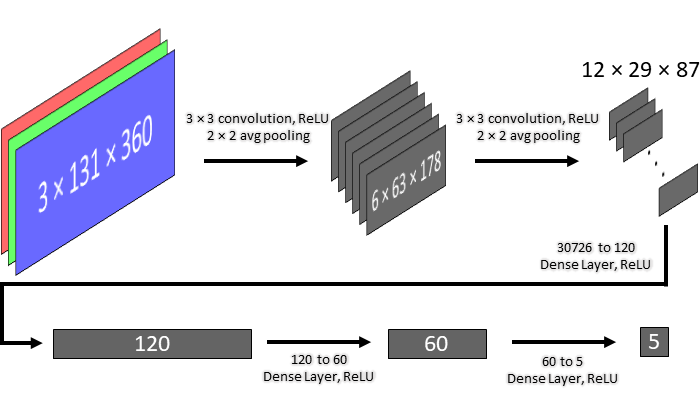
\includegraphics[width=1.0\textwidth]{images/cnnDiag.png}
	\caption{Architecture diagram of our CNN for this problem, beginning with a $3 \times 131 \times 360$ instance and ending with 5 output values corresponding to the class prediction}
	\end{center}
\end{figure}

\subsection{Training}
Our dataset contains only 288 instances; the decision was made to explicitly holdout 38 instances for testing, leaving 250 for training. Holdout was performed on the last entries in the dataset; we make this choice of holdout as opposed to a random sampling or more advanced cross-validation techniques as our data is implicitly ordered by time; we are most interested in performance on future weather events. This is in contrast to more conventional image classification problems whereby instances are unordered and are fully independent, where holdout via random sampling or cross-validation would be more applicable for performance evaluation.

\smallskip

Training was completed using mini-batch gradient descent on randomly sampled batches of size 10 with a constant learning rate of 0.01. This was iterated over a maximum of 250 epochs, with early stopping should the training error fall below 1\%. In summary, there are 25 batches per epoch, for a maximum of $250 \times 25 = 6250$ gradient descent steps in the training process.

\section{Results}
We trained five randomly initialised CNNs for each of our twelve label datasets. Prediction performance on the holdout set is tabulated below in the form of percentage of correctly classified instances; zeroR (the trivial majority class predictor) is included as a benchmark. Since there are 5 distinct labels, the expected performance of random prediction is 20\%.

\begin{center}
\begin{tabular}{|c | r | r | r | r | r | r|}
\hline
\multicolumn{7}{|c|}{Accuracy on Test Data (Average Monthly Rainfall)} \\
\hline
 & ENI & ESI & NNI & NSI & WNI & WSI\\
\hline
1 & 23.684 & 26.315 & 31.578 & 18.421 & \bf28.947 & \bf{36.842} \\
2 & 26.315 & \bf{28.947} & \bf{42.105} & 21.052 & 28.947 & 21.052 \\
3 & 21.053 & 23.684 & 39.473 & 21.052 & 21.052 & 31.578 \\
4 & 28.947 & \bf{28.947} & 36.842 & \bf{23.684} & \bf{42.105} & 31.578 \\
5 & \bf{31.578} & 23.684 & 31.578 & \bf{23.684} & 15.789 & 31.578 \\
\hline
avg & 26.315 & 26.315 & \bf{36.315} & 21.578 & 27.368 & 30.525 \\
\hline
\it{zeroR} & 18.421 & 10.526 & 31.578 & 34.210 & 15.789 & 13.157 \\
\hline
\end{tabular}

\vspace{1cm}

\begin{tabular}{|c | r | r | r | r | r | r|}
\hline
\multicolumn{7}{|c|}{Accuracy on Test Data (Average Monthly Temperature)} \\
\hline
 & ENI & ESI & NNI & NSI & WNI & WSI\\
\hline

1 & 21.052 & 13.157 & 42.105 & 15.789 & 15.789 & 15.789 \\
2 & 26.315 & 21.052 & \bf{50.000} & \bf{36.842} & 21.052 & 10.526 \\
3 & \bf{28.947} & 26.315 & 42.105 & 15.789 & 21.052 & 15.789 \\
4 & 21.052 & 23.684 & 31.578 & 21.052 & \bf{28.947} & 23.684 \\
5 & 23.684 & \bf{31.578} & 28.947 & 26.315 & 21.052 & \bf{26.315} \\
\hline
avg & 24.210 & 23.157 & \bf{38.947} & 23.157 & 21.578 & 18.420 \\
\hline
\it{zeroR} & 13.157 & 18.421 & 18.421 & 28.947 & 0.000 & 10.526 \\
\hline
\end{tabular}
\end{center}
\begin{figure}[h]
	\begin{center}
	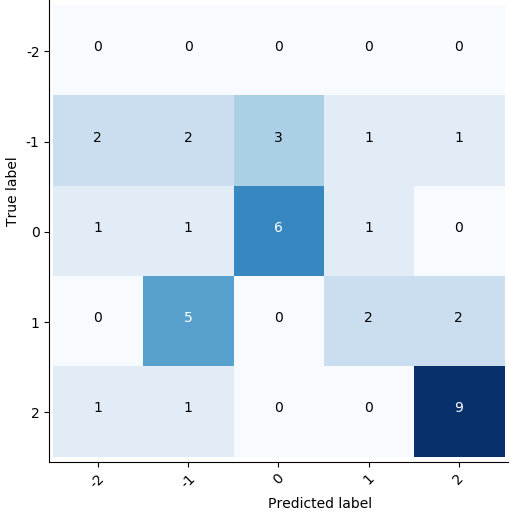
\includegraphics[width=8cm]{images/confusion1}
	\caption{Confusion matrix of best trial (NNI TMean, 50\% acc.)}
	\end{center}
\end{figure}

\pagebreak

\section{Evaluation}
\subsection{Performance}
The results of testing shows that this CNN implementation marginally outperforms zeroR and random guessing. Interestingly, zeroR failing to outperform a baseline 20\% accuracy expected from random guessing in many of the cases indicates that historical label data is a poor predictor of future labels. The NNI dataset displays the best performance for both temperature and rainfall; this may be an indication that the correlation of GCMs and northern New Zealand observations is greater than other areas. Although this model outperforms trivial baselines, it is not an overall effective predictor of monthly weather patterns in New Zealand, as it fails to achieve 50\% performance in even the best cases, meaning the output is more often wrong than right.

\subsection{Data Quality}
The small size of our dataset may have contributed to poorer performance of this model; we have only 250 training instances, whereas MNIST and CIFAR-10 uses 60000. Moreover, these traditional datasets have uniform class distributions (that is, there are 6000 images for each of the 10 possible labels) whereas our dataset does not; recall that the quintile definition used as the class label in our dataset is based on a wider population and hence does not divide instances into five equally sized sets. 

\subsection{Data Visualisation}
Recall that our GCM tensors were normalised to values between 0 and 1. By multiplying each entry by 255 and then rounding to the nearest integer, it is possible to visualise our GCMs as standard 8-bit grey-scale images (Figure 3). Stacking these as channels of an RGB image gives us a 24-bit colour image best representing a single input instance (Figure 4). We note that, unlike traditional image classification challenges, our input images are not human readable; whereas we could reasonably expect a human to recognise MNIST images and correctly classify them as digits, the same expectation does not apply to classifying our GCM image into the correct quintile for some climate variable in a region of New Zealand. This may be the reason the same performance cannot be reached in this problem as compared to those achieved on CNNs for MNIST, CIFAR-10, and other "human-recognisable" image recognition tasks; the correlation between GCM outputs and local weather variables are more latent.
\pagebreak

\begin{figure}[h]
	\begin{center}
	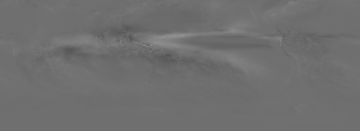
\includegraphics[width=8cm]{images/Figure_1}
	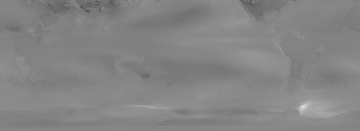
\includegraphics[width=8cm]{images/Figure_2}
	
\includegraphics[width=8cm]{images/Figure_3}
	\caption{Greyscale visualisations of GCM precipitation, temperature, geopotential (top to bottom)}
	\end{center}
\end{figure}
\begin{figure}[h]
	\begin{center}
	
\includegraphics[width=8cm]{images/Figure_RGB}
	\caption{All three input GCM channels combined into single RGB image}
	\end{center}
\end{figure}

\subsection{Possible Improvements}
The small size of this dataset meant no held-out validation set was used to measure performance during the training process; instead the choice was made to naively implement early stopping upon reaching rote-performance on the training data. A dedicated validation set with early stopping on non-monotonic decrease of error rate may possibly reduce over-fitting on future experiments.

\smallskip

One possible way to address our data having non-uniform class label counts may be to duplicate instances with less commonly occurring labels to ensure uniformity; \cite{buda2018systematic} shows that this simple approach to resolve the class imbalance problem yields good prediction performance.

\smallskip

The "cat5" class label was derived from discretizing continuous values into bins with respect to quintiles from a larger dataset by NIWA. Predicting this label rather than regressing the original continuous values allowed for the classification based solution used in this project. However, by applying this approach, we make the simplification that our labels are unordered; this simplification may impair predictive performance, as our model fails to consider the ordinality of our label data - clearly, the cat5 bins are ordered $-2 < -1 < 0 < 1 < 2$ as they represent intervals of the original continuous values. \cite{frank2001simple} proposes a solution by transforming ordinal classification problems into a set of binary-class type problems, whereby labels in each problem are a true or false based on whether or not the label exceeds a given threshold; in our case, this would correspond to four new binary labels - [cat5 $>$ 1], [cat5 $>$ 0] , [cat5 $>$ -1], and [cat5 $>$ -2].

\smallskip

Our GCM data used an equirectangular projection of the Earth's surface onto a plane. This projection maps a spherical coordinate system to a cartesian coordinate system without transformation (or equivalently, under the identity transformation). Hence for any $x, y$ on the transformed image $$(x, y) =(\theta, \phi)$$ where $\theta$ is longitude and $\phi$ is latitude on the Earth in degrees. This projection does not preserve area; a constant change in longitude does not correspond to a constant change of distance but depends on the distance from the equator. Polar regions are therefore implicitly weighted higher, which is a behaviour we do not want during the training process. GCMs with a different choice of transformation may yield better results; additionally, previous work has also been carried out in image recognition for spherical coordinate systems in the context of $360^{\circ}$ cameras \cite{su2017learning}.



\section{Conclusion}
The objective of this project was to use Convolutional Neural Networks to predict the cat5 label of monthly weather variables in New Zealand using Global Circulation Model outputs. The motivation behind this was due to the analogue of this problem to traditional image classification problems. While our model outperforms trivial baselines, it fails to approach the same level of performance achieved by CNNs on conventional datasets such as MNIST, CIFAR-10, and FashionMNIST. A combination of factors such as a small dataset size, naive validation method, discarding information regarding ordinality of the labels, and failure to account for the non-conformal equirectangular projection that our dataset uses may have contributed to poor predictive performance. We note that the correlation between GCM and quintile label is not reasonably human-recognisable and more latent than other image recognition tasks, which may explain its higher difficulty.

\pagebreak

\bibliography{final}
\bibliographystyle{apalike}

\end{document}